\subsection{Ca sử dụng gửi tin nhắn}
\vspace{0.5cm}


\noindent 
\begin{tabularx}{\linewidth}{| l | X |} 
\hline 
\textbf{Mô tả} & Người dùng có thể gửi tin nhắn trong nhóm hoặc gửi tin nhắn riêng cho bạn bè.  \\ 
\hline 
\textbf{Luồng cơ bản} & 1. Người dùng truy cập tab tin nhắn. \newline
                        2. Người dùng bấm vào một cuộc hội thoại muốn gửi tin nhắn. \newline
                        3. Hệ thống hiển thị thông tin của cuộc hội thoại và các tin nhắn trong cuộc hội thoại đó. \newline
                        4. Người dùng nhập tin nhắn muốn gửi. \newline
                        5. Người dùng bấm gửi. \newline
                        6. Hệ thống gửi tin nhắn và hiển thị tin nhắn vừa gửi lên cuộc hội thoại. \\
                        
\hline 
\textbf{Luồng thay thế} & Người dùng đính kèm địa điểm vào tin nhắn \newline
   1. Người dùng nhấn nút "+" cạnh ô input. \newline
   2. Hệ thống hiển thị giao diện tìm kiếm/chọn địa điểm. \newline
   3. Người dùng chọn một địa điểm. \newline
   4. Hệ thống thêm thông tin địa điểm đã chọn vào nội dung tin nhắn đang soạn thảo. \\

                       
\hline 
\textbf{Tiền điều kiện} &- Người dùng đang đăng nhập và phiên đăng nhập chưa kết thúc. \newline
                        - Người dùng đã có ít nhất một cuộc hội thoại. \\
\hline 
\textbf{Hậu điều kiện} & - Hệ thống lưu tin nhắn vào cơ sở dữ liệu và hiển thị tin nhắn trong cuộc hội thoại trong thời gian thực. \newline
                        - Hệ thống nhận diện địa điểm trong tin nhắn và highlight các địa điểm đó. \newline
                        - Hệ thống phân loại tin nhắn có cần thiết cho tổng hợp lịch trìn hay không. \newline
                        - Người dùng có thể nhấn vào địa điểm trong tin nhắn để xem chi tiết địa điểm. \newline
                        - Người dùng có thể react hoặc gỡ tin nhắn\\

\hline 
\textbf{Yêu cầu phi chức năng} & Hệ thống xử lý gửi tin nhắn dưới 1s  \\ 
\hline 
\end{tabularx}



\noindent 
\begin{tabular}{| c | c |}
    \hline
    \textbf{Biểu đồ hoạt động} & \textbf{Quan hệ} \\ 
    \hline
    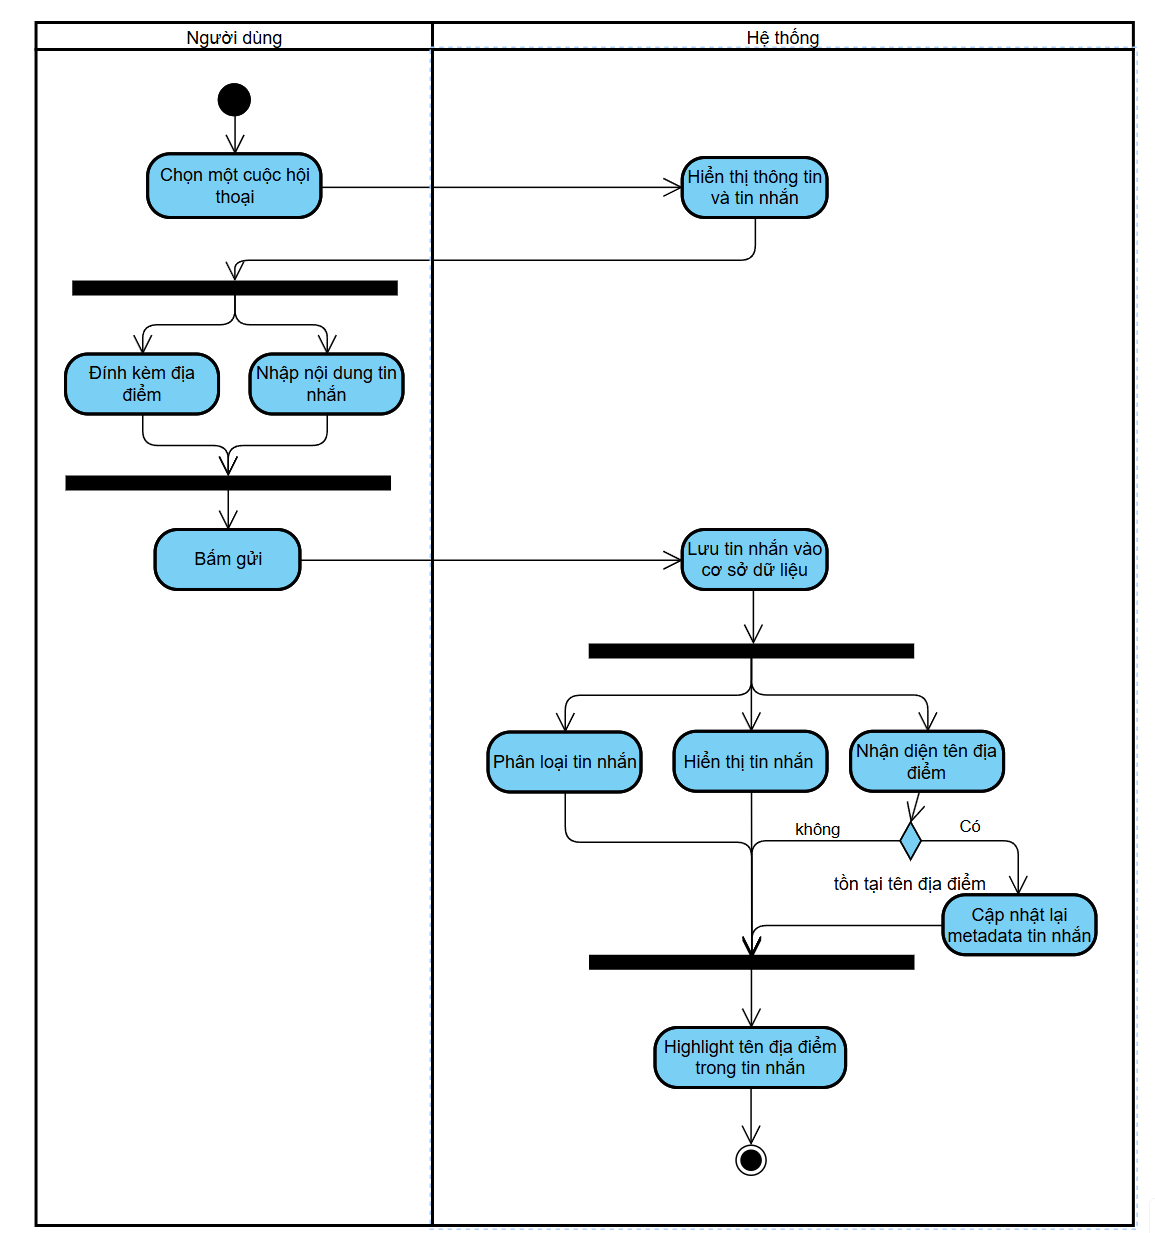
\includegraphics[width=0.5\linewidth]{figures/c3/3-3-9-ad.png} 
    & 
    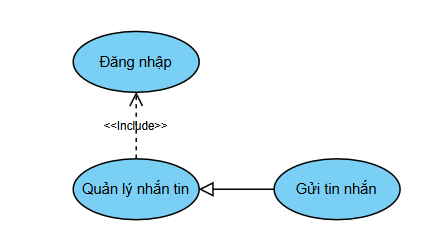
\includegraphics[width=0.45\linewidth]{figures/c3/3-3-9-rd.png} \\ 
    \hline
\end{tabular}


\vspace{0.8cm}

\begin{figure}[H]
    \centering  
    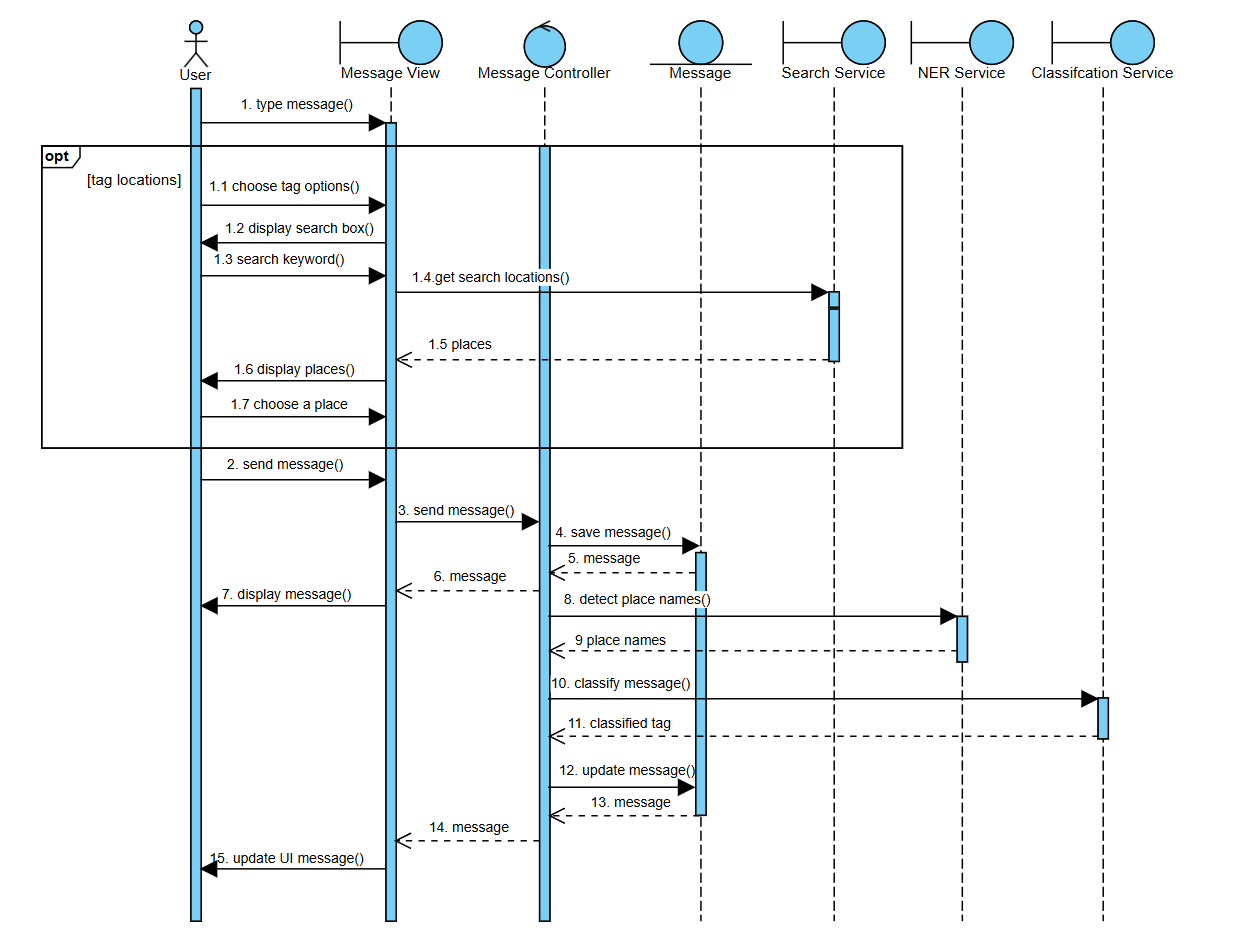
\includegraphics[width=1\textwidth]{figures/c3/3-3-9-sd.png}
    \caption{Biểu đồ tuần tự ca sử dụng gửi tin nhắn.}
    \label{fig:3-3-9-sequence-diagram}
\end{figure}